\documentclass{article}
\usepackage{graphicx} % Required for inserting images
\usepackage{minted}
\usepackage{array}

\title{Circuitos Digitais I - Atividades 1-3: Aulas 2-3}
\author{Luis Felipe Ferreira Soares}
\date{Outubro 2025}

\begin{document}

\maketitle

\section*{Atividade 1}
\setcounter{section}{1}
\setcounter{subsection}{0}

\subsection{Conversor estrutural BCD5311 para BCD8421}
\begin{minted}{verilog}
module d_module (
    input h, g, f, e,
    output d
);

and A1(d, h, g);

endmodule

module c_module (
    input h, g, f, e,
    output c
);

wire h_, g_, w1, w2;

not N1(g_, g);
not N2(h_, h);
and A1(w1, h_, g, e);
and A2(w2, h, g_);
or O1(c, w1, w2);

endmodule

module b_module (
    input h, g, f, e,
    output b
);

wire h_, g_, e_, w1, w2, w3;

not N1(g_, g);
not N2(h_, h);
not N3(e_, e);
and A1(w1, h_, g, e_);
and A2(w2, g_, f);
and A3(w3, h, g_);
or O1(b, w1, w2, w3);

endmodule

module a_module (
    input h, g, f, e,
    output a
);

wire h_, g_, f_, e_, w1, w2, w3, w4, w5;

not N1(h_, h);
not N2(g_, g);
not N3(f_, f);
not N4(e_, e);
and A1(w1, h_, g_, e, f_);
and A2(w2, h_, g, e_);
and A3(w3, g, f);
and A4(w4, h, g, e);
and A5(w5, h, f);
or O1(a, w1, w2, w3, w4, w5);

endmodule

module hfge2dcba (
    input h, g, f, e,
    output d, c, b, a
);

d_module D(h, g, f, e, d);
c_module C(h, g, f, e, c);
b_module B(h, g, f, e, b);
a_module A(h, g, f, e, a);

endmodule
\end{minted}

\newpage
\subsection{Testbench}
\begin{minted}{verilog}
module hfge2dcba_tb;
reg h, g, f, e;
wire d, c, b, a;

hfge2dcba dut (h, g, f, e, d, c, b, a);

initial begin
    $display("HGFE | DCBA");
    $monitor("%b%b%b%b | %b%b%b%b", h, g, f, e, d, c, b, a);
    {h,g,f,e} = 4'b0000; #10;
    {h,g,f,e} = 4'b0001; #10;
    {h,g,f,e} = 4'b0011; #10;
    {h,g,f,e} = 4'b0100; #10;
    {h,g,f,e} = 4'b0101; #10;
    {h,g,f,e} = 4'b0111; #10;
    {h,g,f,e} = 4'b1001; #10;
    {h,g,f,e} = 4'b1011; #10;
    {h,g,f,e} = 4'b1100; #10;
    {h,g,f,e} = 4'b1101; #10;
end

endmodule
\end{minted}

\subsection{Console output}
\begin{verbatim}
HGFE | DCBA
0000 | 0000
0001 | 0001
0011 | 0010
0100 | 0011
0101 | 0100
0111 | 0101
1001 | 0110
1011 | 0111
1100 | 1000
1101 | 1001
\end{verbatim}

\subsection{Conversor BCD5311 para BCD8421 - Portas Lógicas}
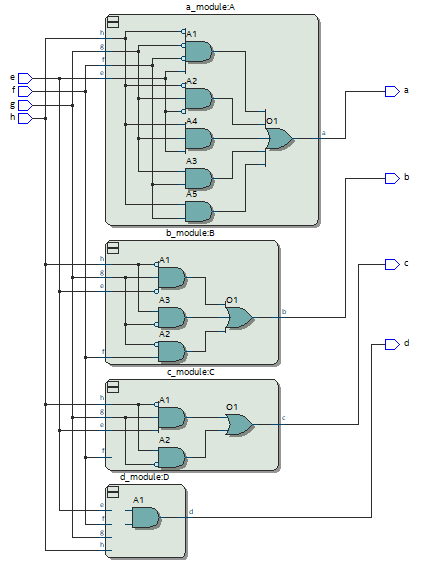
\includegraphics[width=1\textwidth]{hgfe_rtl.png}

\subsection{Conversor BCD5311 para BCD8421 - Simulação}
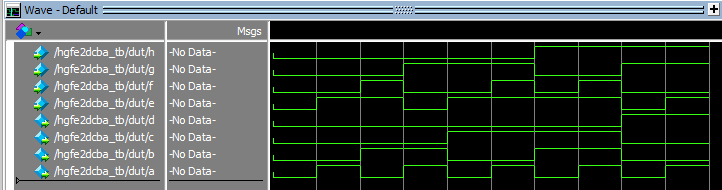
\includegraphics[width=1\textwidth]{hgfe_wave.png}

\setcounter{section}{2}
\setcounter{subsection}{0}
\section*{Atividade 2}
\subsection{Tabela verdade do conversor BCD8421 para Excesso de 3}
$$\begin{array}{|c|c c c c|c c c c|} \hline \mathbf{N} & \mathbf{A} & \mathbf{B} & \mathbf{C} & \mathbf{D} & \mathbf{W} & \mathbf{X} & \mathbf{Y} & \mathbf{Z} \\ \hline 0 & 0 & 0 & 0 & 0 & 0 & 0 & 1 & 1 \\ 1 & 0 & 0 & 0 & 1 & 0 & 1 & 0 & 0 \\ 2 & 0 & 0 & 1 & 0 & 0 & 1 & 0 & 1 \\ 3 & 0 & 0 & 1 & 1 & 0 & 1 & 1 & 0 \\ 4 & 0 & 1 & 0 & 0 & 0 & 1 & 1 & 1 \\ 5 & 0 & 1 & 0 & 1 & 1 & 0 & 0 & 0 \\ 6 & 0 & 1 & 1 & 0 & 1 & 0 & 0 & 1 \\ 7 & 0 & 1 & 1 & 1 & 1 & 0 & 1 & 0 \\ 8 & 1 & 0 & 0 & 0 & 1 & 0 & 1 & 1 \\ 9 & 1 & 0 & 0 & 1 & 1 & 1 & 0 & 0 \\ \hline 10 & 1 & 0 & 1 & 0 & X & X & X & X \\ 11 & 1 & 0 & 1 & 1 & X & X & X & X \\ 12 & 1 & 1 & 0 & 0 & X & X & X & X \\ 13 & 1 & 1 & 0 & 1 & X & X & X & X \\ 14 & 1 & 1 & 1 & 0 & X & X & X & X \\ 15 & 1 & 1 & 1 & 1 & X & X & X & X \\ \hline \end{array}$$

\subsection{Mapa de Karnaugh}
\begin{center}
\begin{tabular}{>{\centering\arraybackslash}m{0.45\textwidth}>{\centering\arraybackslash}m{0.45\textwidth}}
% Célula 1: Saída W
\begin{minipage}[t]{\linewidth}
    \centering
    % Equação
    $$W = A + BD + BC$$ 
    % Imagem
    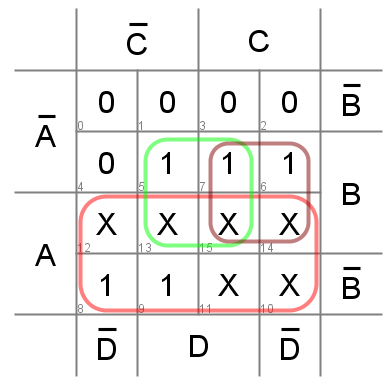
\includegraphics[width=0.8\linewidth]{xs3-kmap-W.png}
\end{minipage}
&
% Célula 2: Saída X
\begin{minipage}[t]{\linewidth}
    \centering
    % Equação
    $$X = B'D + B'C + BC'D'$$ 
    % Imagem
    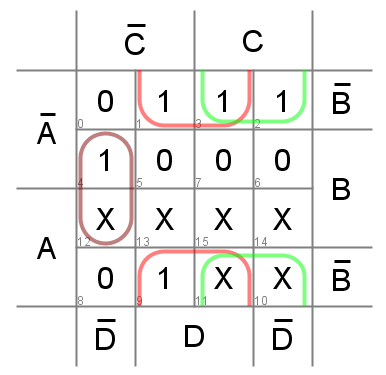
\includegraphics[width=0.8\linewidth]{xs3-kmap-X.png}
\end{minipage}
\\
% Célula 3: Saída Y
\begin{minipage}[t]{\linewidth}
    \centering
    % Equação
    $$Y = C'D' + CD$$
    % Imagem
    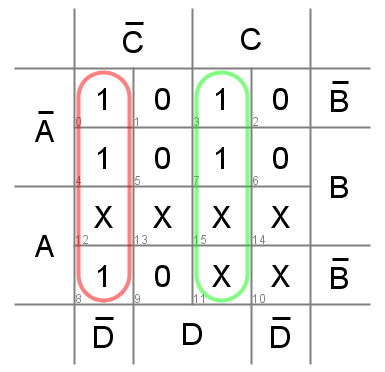
\includegraphics[width=0.8\linewidth]{xs3-kmap-Y.png}
\end{minipage}
&
% Célula 4: Saída Z
\begin{minipage}[t]{\linewidth}
    \centering
    % Equação
    $$Z = D'$$
    % Imagem
    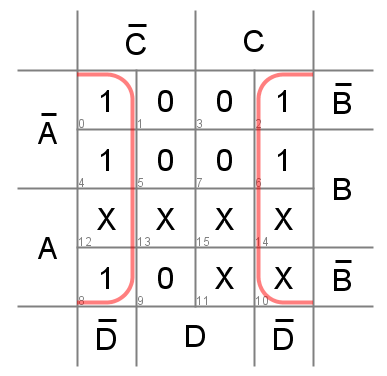
\includegraphics[width=0.8\linewidth]{xs3-kmap-Z.png}
\end{minipage}
\\
\end{tabular}
\end{center}

\subsection{Código do conversor - Descrição RTL/Fluxo de dados}
\begin{minted}{verilog}
module bcd2xs3 (
    input a, b, c, d,
    output w, x, y, z
);

assign w = a | b & d | b & c;
assign x = !b & d | !b & c | b & !c & !d;
assign y = !c & !d | c & d;
assign z = !d;

endmodule
\end{minted}

\subsection{Testbench}
\begin{minted}{verilog}
module bcd2xs3_tb;
reg a, b, c, d;
wire w, x, y, z;

bcd2xs3 dut (a, b, c, d, w, x, y, z);

initial begin
    $display("ABCD | WXYZ");
    $monitor("%b%b%b%b | %b%b%b%b", a, b, c, d, w, x, y, z);
    {a,b,c,d} = 4'b0000; #10;
    {a,b,c,d} = 4'b0001; #10;
    {a,b,c,d} = 4'b0010; #10;
    {a,b,c,d} = 4'b0011; #10;
    {a,b,c,d} = 4'b0100; #10;
    {a,b,c,d} = 4'b0101; #10;
    {a,b,c,d} = 4'b0110; #10;
    {a,b,c,d} = 4'b0111; #10;
    {a,b,c,d} = 4'b1000; #10;
    {a,b,c,d} = 4'b1001; #10;
end

endmodule
\end{minted}

\subsection{Console output}
\begin{verbatim}
ABCD | WXYZ
0000 | 0011
0001 | 0100
0010 | 0101
0011 | 0110
0100 | 0111
0101 | 1000
0110 | 1001
0111 | 1010
1000 | 1011
1001 | 1100
\end{verbatim}

\subsection{Conversor BCD8421 para Excesso de 3 - Portas lógicas}
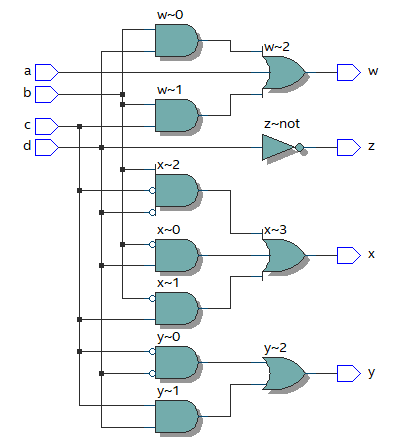
\includegraphics[width=1\textwidth]{xs3-rtl.png}

\subsection{Conversor BCD8421 para Excesso de 3 - Simulação}
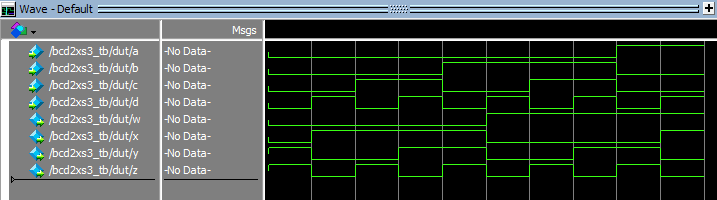
\includegraphics[width=1\textwidth]{xs3-wave.png}

\setcounter{section}{3}
\setcounter{subsection}{0}
\section*{Atividade 3}
\subsection{Mapa de Karnaugh}

\begin{center}
\begin{tabular}{>{\centering\arraybackslash}m{0.45\textwidth}>{\centering\arraybackslash}m{0.45\textwidth}}
% Célula 1: Saída W
\begin{minipage}[t]{\linewidth}
    \centering
    % Equação
    $$W = A$$
    % Imagem
    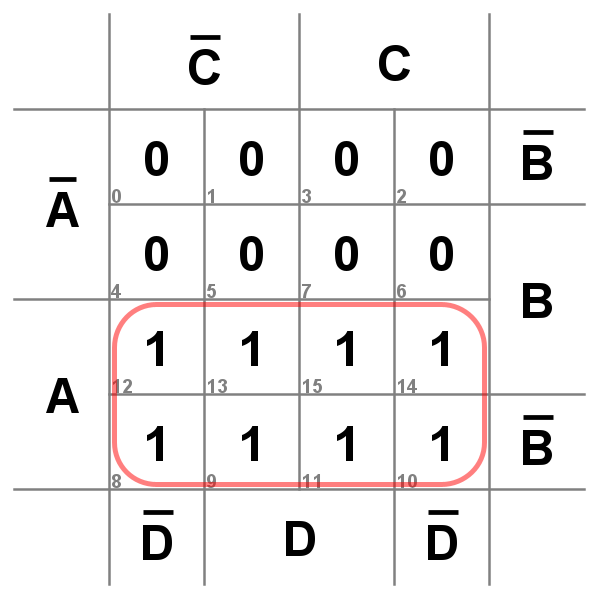
\includegraphics[width=0.8\linewidth]{bcd2gray-W.png}
\end{minipage}
&
% Célula 2: Saída X
\begin{minipage}[t]{\linewidth}
    \centering
    % Equação
    $$X = A'B + AB'$$ 
    % Imagem
    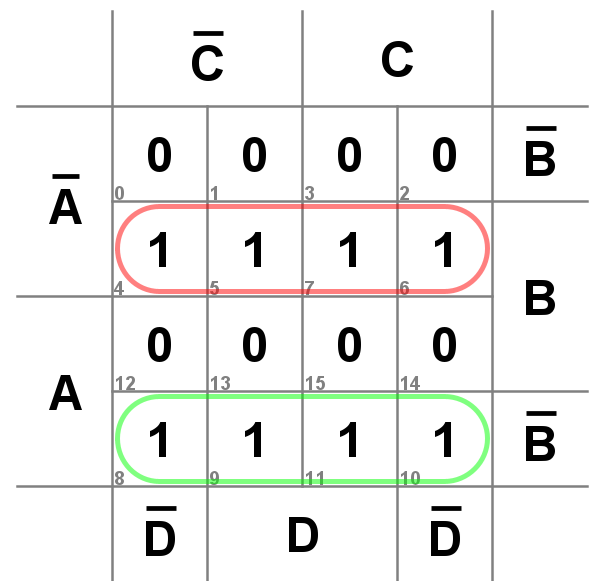
\includegraphics[width=0.8\linewidth]{bcd2gray-X.png}
\end{minipage}
\\
% Célula 3: Saída Y
\begin{minipage}[t]{\linewidth}
    \centering
    % Equação
    $$Y = B'C + BC'$$
    % Imagem
    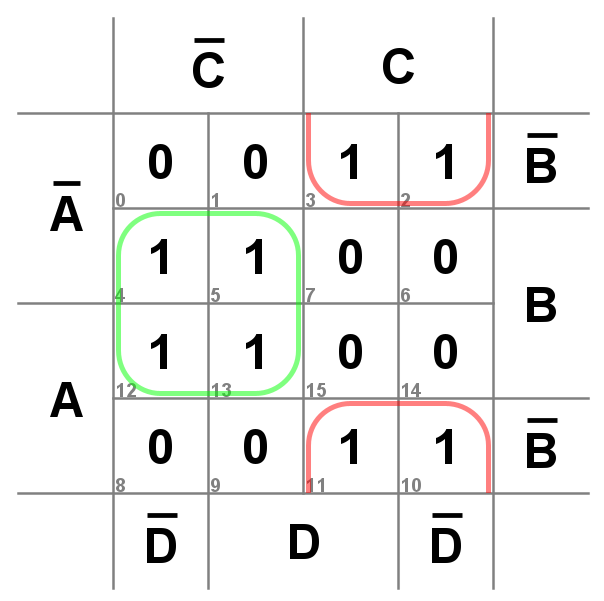
\includegraphics[width=0.8\linewidth]{bcd2gray-Y.png}
\end{minipage}
&
% Célula 4: Saída Z
\begin{minipage}[t]{\linewidth}
    \centering
    % Equação
    $$Z = C'D + CD'$$
    % Imagem
    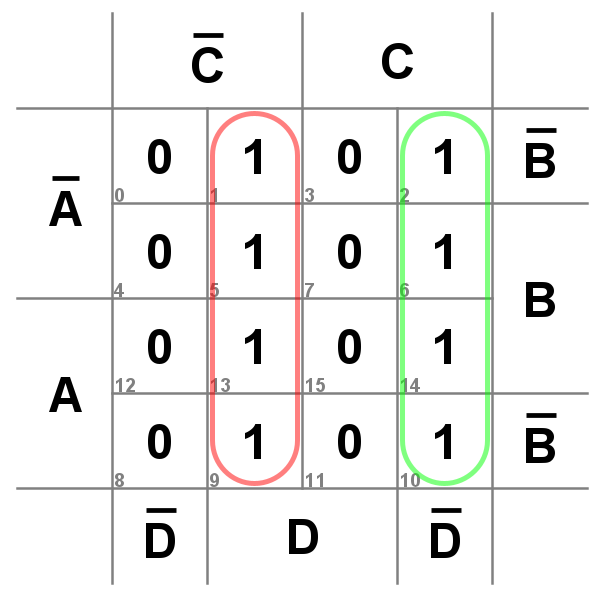
\includegraphics[width=0.8\linewidth]{bcd2gray-Z.png}
\end{minipage}
\\
\end{tabular}
\end{center}

\subsection{Código do conversor BCD8421 para Código Gray}
\begin{minted}{verilog}
module bcd2gray (
    input a, b, c, d,
    output w, x, y, z
);

assign w = a;
assign x = !a & b | a & !b;
assign y = !b & c | b & !c;
assign z = !c & d | c & !d;

endmodule
\end{minted}

\subsection{Testbench}
\begin{minted}{verilog}
module bcd2gray_tb;
reg a, b, c, d;
wire w, x, y, z;

// para agrupamento na visualização apenas
wire [3:0] bcd, gray;
assign bcd = {a, b, c, d};
assign gray = {w, x, y, z};

bcd2gray dut(a, b, c, d, w, x, y, z);

always #1 d = !d;
always #2 c = !c;
always #4 b = !b;
always #8 a = !a;

initial begin
    $display("ABCD | WXYZ");
    $monitor("%b%b%b%b | %b%b%b%b", a, b, c, d, w, x, y, z);
    {a, b, c, d} = 4'b0000;
    #16 $finish;
end

endmodule
\end{minted}

\subsection{Console output}
\begin{verbatim}
ABCD | WXYZ
0000 | 0000
0001 | 0001
0010 | 0011
0011 | 0010
0100 | 0110
0101 | 0111
0110 | 0101
0111 | 0100
1000 | 1100
1001 | 1101
1010 | 1111
1011 | 1110
1100 | 1010
1101 | 1011
1110 | 1001
1111 | 1000
\end{verbatim}

\subsection{Conversor BCD8421 para Código Gray - Portas lógicas}
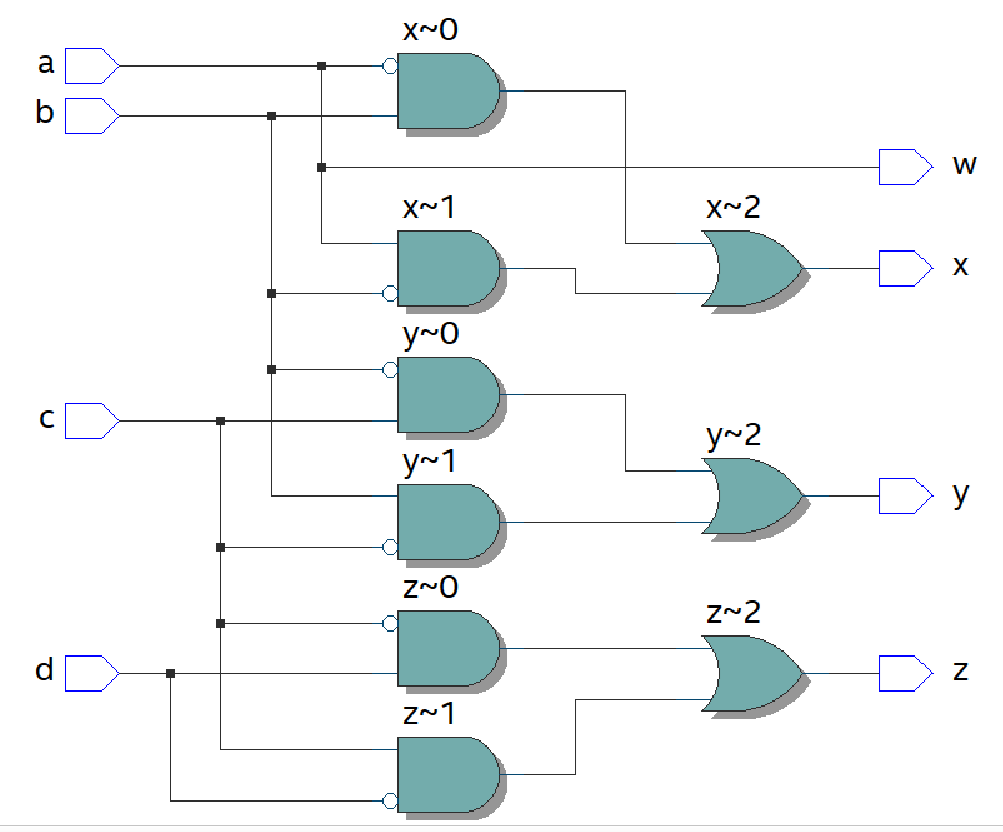
\includegraphics[width=1\textwidth]{bcd2gray-rtl.png}

\subsection{Conversor BCD8421 para Código Gray - Portas lógicas}
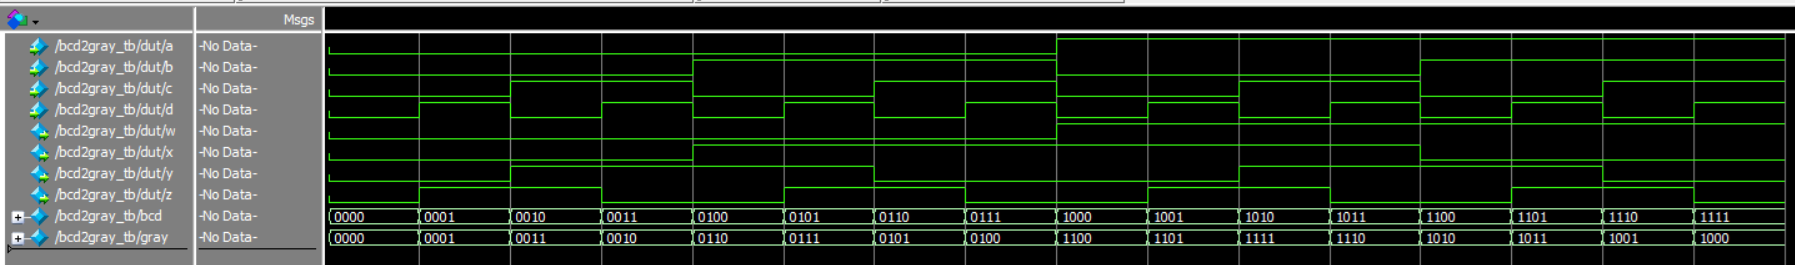
\includegraphics[width=1\textwidth]{bcd2gray-wave.png}

\end{document}